\section{Пример: данные по гормонам}

В таблице 9.1 показан небольшой набор данных, который является подходящим для регрессионного анализа. Медицинское устройство для непрерывной доставки противовоспалительного гормона было протестировано на $27$ пациентах. Переменная ответа $y_i$ --- это количество гормона, оставшееся в устройстве после ношения,
$$y_i = \text{ оставшееся количество гормона в устройстве } i, \; i = 1, 2, \ldots, 27.$$
Есть две переменные--предикторы,
$$z_i = \text{ количество часов ношения i-го устройства}$$
и
$$L_i = \text{ производственная партия устройства i}.$$
Тестируемые устройства были случайным образом выбраны из трех различных производственных партий, названных $A$, $B$ и $C$.

Левая часть рисунка 9.1 представляет собой диаграмму рассеяния 27 точек $(z_i, y_i) = (\text{часы}_i, \text{число}_i)$ с символом $L_i$, используемым в качестве графического сивола. Мы видим, что более длительное время ношения приводит к меньшему количеству оставшегося гормона, как и следовало ожидать. Мы можем количественно оценить это наблюдение с помощью регрессионного анализа.

Рассмотрим модель, в которой математическое ожидание $y$ является линейной функцией $z$,
\begin{equation}
	\mu_i = \text{E}(y_i|z_i) = \beta_0 + \beta_1 z_i \quad i = 1,2, \ldots, 27.
\end{equation}
Эта модель игнорирует $L_i$: она имеет форму (9.3) с векторами признаков размерности $p = 2$,
\begin{equation}
	\textbf{c}_i = (1, z_i).
\end{equation}
Вектор неизвестных параметров $\bm{\beta}$ был помечен $(\beta_0, \beta_1)$ вместо $(\beta_1, \beta_2)$, так что индексы соответствуют степеням $z$, как в (7.20). Нормальные уравнения (9.10) дают оценку по методу наименьших квадратов
\begin{equation}
	\hat{\bm{\beta}} = (34.17, -0.0574)^\text{T}.
\end{equation}
Линия регрессии, оцененная методом наименьших квадратов
\begin{equation}
	\hat{\mu}_i = \textbf{c}_i \hat{\bm{\beta}} = \hat{\beta}_0 + \hat{\beta}_1 z_i
\end{equation}
изображена на правой части рисунка 9.1. Среди всех возможных линий, которые можно было нарисовать, эта линия минимизирует сумму квадратов $27$ вертикальных расстояний от точек до линии.

Насколько точен оценочный вектор параметров $\hat{\bm{\beta}}$? Ответ дает чрезвычайно полезная формула, также восходящая к Лежандру и Гауссу. Пусть $\textbf{G}$ --- матрица скалярных произведений $p \times p$,
\begin{equation}
	\textbf{G} = \textbf{C}^\text{T}\textbf{C},
\end{equation}
матрица с элементом $g_{hj} = \sum\limits_{i=1}^{n} c_{ih} c_{ij}$ в строке $h$, столбце $j$. Пусть $\sigma^2_F$ будет дисперсией ошибок в модели (9.4),
\begin{equation}
	\sigma^2_F = \text{var}_F(\varepsilon).
\end{equation}

Тогда стандартная ошибка $j$-го компонента $\hat{\bm{\beta}}$, квадратного корня из его дисперсии, равна
\begin{equation}
	\text{se}(\hat{\beta}_j) = \sigma_F \sqrt{G^{jj}}
\end{equation}
где $G^{jj}$ --- $j$-й диагональный элемент обратной матрицы $\textbf{G}^{-1}$.

\noindent
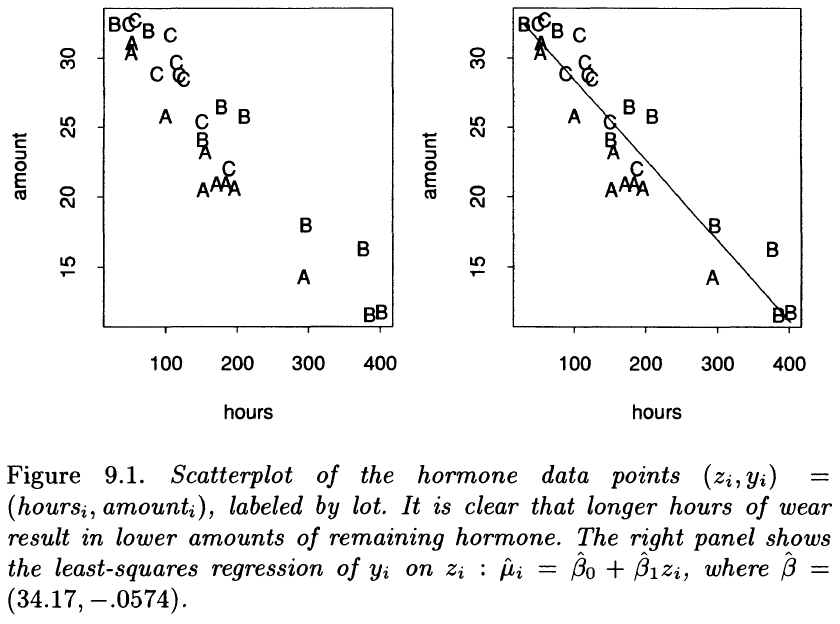
\includegraphics[width=\linewidth]{9/f91}
\newline

Последняя формула является обобщением формулы (5.4) для стандартной ошибки выборочного среднего, $\text{se}_F(\bar{x}) = \sigma_F / \sqrt{n}$, см. задачу 9.1. На практике $\sigma_F$ оценивается по формуле, аналогичной (5.11),
\begin{equation}
	\hat{\sigma}_F = \left\{ \sum\limits_{i=1}^{n} (y_i - \textbf{c}_i \hat{\bm{\beta}})^2 / n \right\}^{1/2} = \{ \text{RSE}(\hat{\bm{\beta}})/n \}^{1/2}
\end{equation}
или версией $\hat{\sigma}_F$ с корректированным смещением,
\begin{equation}
	\bar{\sigma}_F = \{ \text{RSE}(\hat{\bm{\beta}})/(n-p) \}^{1/2}.
\end{equation}
Соответствующие оценочные стандартные ошибки для компонентов $\hat{\bm{\beta}}$ равны
\begin{equation}
	\widehat{\text{se}}(\hat{\beta}_j) = \hat{\sigma}_F \sqrt{G^{jj}} \quad \text{или} \quad \overline{\text{se}} (\hat{\beta}_j) = \hat{\sigma}_F \sqrt{G^{jj}}.
\end{equation}
Связь между $\widehat{\text{se}}(\hat{\beta}_j)$ и $\overline{\text{se}}(\hat{\beta}_j)$ такая же, как между формулами (5.12) и (2.2) для среднего.

\noindent
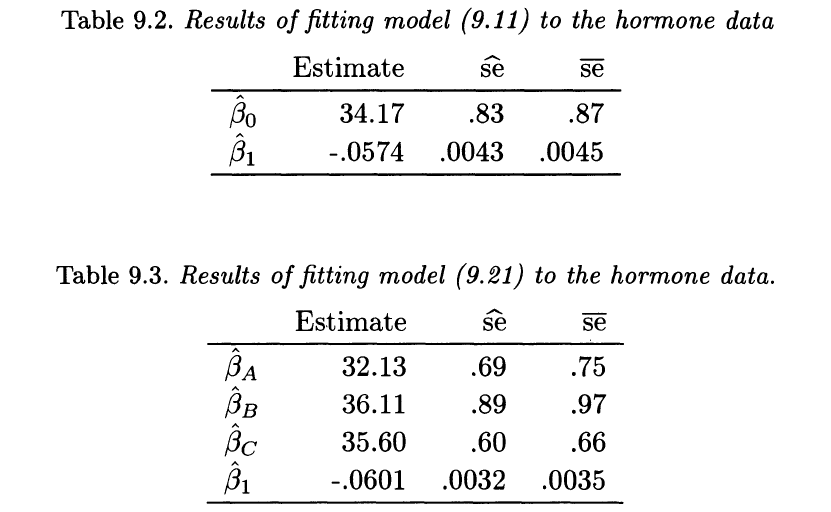
\includegraphics[width=\linewidth]{9/t92t93}
\newline

Большинство программ для линейной регрессии с библиотеками обычно выдают результат $\bar{\text{se}}(\hat{\beta}_j)$ вместе с оценкой $\hat{\beta}_j$ методом наименьших квадратов. Применение такой программы к модели (9.11) для данных по гормону дает результаты в таблице 9.2.

Глядя на правую часть рисунка 9.1, большинство точек для партии $A$ лежат ниже подобранной линии регрессии, в то время как большинство точек для партий $B$ и $C$ лежат выше этой линии. Это говорит о неточности модели (9.11). Если бы модель была точной, можно было бы ожидать, что примерно половина каждой партии будет лежать выше, а половина ниже установленной линии. Выражаясь обычной терминологией, похоже, что в данных присутствует эффект партии.

В нашу линейную модель легко включить эффект партии. Мы предполагаем, что условное математическое ожидание $y$ при заданных $L$ и $z$ имеет вид
\begin{equation}
	\text{E}(y|L,z) = \beta_L + \beta_1 z.
\end{equation}
Здесь $B_L$ равно одному из трех возможных значений: $\beta_A, \beta_B, \beta_C$, в зависимости от партии устройства. Это похоже на модель (9.11), за исключением того, что (9.21) допускает разные точки пересечения для каждой партии, а не одну точку пересечения $\beta_0$ из (9.11). Анализ модели (9.21) методом наименьших квадратов дал результаты в таблице 9.3.

Обратите внимание, что $\hat{\beta}_A$ на несколько стандартных ошибок меньше чем $\hat{\beta}_B$ и $\hat{\beta}_C$, что указывает на то, что устройства в партии $A$ содержат значительно меньше гормона.